\begin{frame}{The template has a software-style source structure}
\begin{columns}[T,onlytextwidth]
\column{0.50\textwidth}
\centering
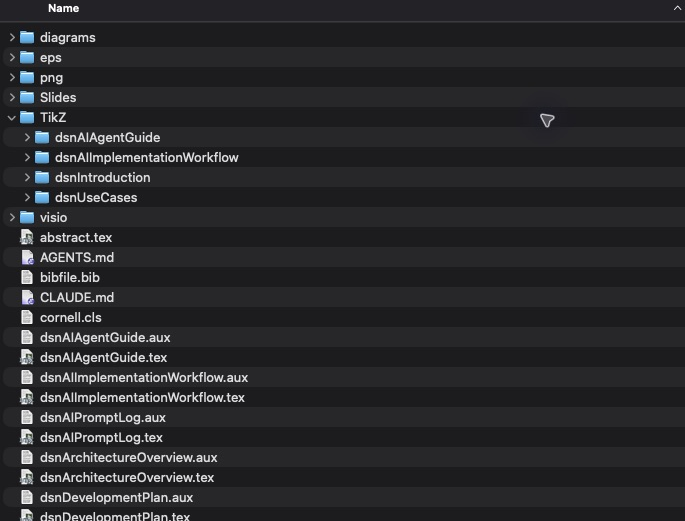
\includegraphics[width=\linewidth,height=5.0cm,keepaspectratio]{assets/dsnTemplateFileStructure.png}
\par\vspace{0.08cm}
{\scriptsize Actual DSN \texttt{main/} folder; Finder screenshot (excerpt).}
\column{0.47\textwidth}
\small
\textbf{Entry point}\par
\texttt{dsnManual.tex} assembles the chapters.
\vspace{0.18cm}

\textbf{Modules}\par
\texttt{dsnRequirements.tex}, \texttt{dsnLogicalView.tex}, etc. own chapter content.
\vspace{0.18cm}

\textbf{Shared diagram sources}\par
\texttt{TikZ/dsnIntroduction/}, etc. organize diagrams by chapter; slides reuse them.
\vspace{0.18cm}

\textbf{Build and presentation}\par
\texttt{makefileMacLinux} and \texttt{makefilePowerShell.ps1} build the manual; \texttt{Slides/} holds this deck.
\end{columns}
\end{frame}
\note{Screenshot captured from the actual ArchitectureDesignTemplate/main directory. It is cropped to the file list for legibility. This is an excerpt, not a complete directory inventory; the entry point and build scripts are elsewhere in the same directory. The .aux files visible in Finder are generated build intermediates. Editable chapter and TikZ sources remain authoritative, and the slide deck reuses the corresponding chapter diagrams.}
